\documentclass[logo,reportComp]{thesis}
\usepackage[cpp,pseudo]{mypackage}

\title{高级编程技术实验报告}
\subtitle{实验三:机器人}
\school{数据科学与计算机学院}
\author{陈鸿峥}
\classname{17大数据与人工智能}
\stunum{17341015}
\headercontext{高级编程技术实验报告}
% \authorremark{本实验报告用\LaTeX撰写,创建时间:\builddate\today}
\lstset{language=python}

\begin{document}

\maketitle

\section{问题描述及求解思路}
\subsection{问题一:实施房间与机器人基类}
\verb'RectangularRoom'基类:
\begin{itemize}
    \item \verb'__init__':直接设置\verb'width'和\verb'height'即可,这里要注意尽管\verb'width'和\verb'height'题目中说了是整数,但是在问题六中却输入了一个浮点数,因此在最开始应该先对这两个值取整,以确保后面初始化的正确性。
    同时创建一个\verb'tiles'列表,存储每个格的脏物数,每个格的坐标以左下角的坐标作为下标。
    如正方形格$(1,1),(2,1),(2,2),(1,2)$,存储在\verb'tiles[1][1]'中。
    \item \verb'clean_tile_at_position':先用\verb'pos.get_x()'和\verb'pos.get_y()'取出坐标,注意要\textbf{用}\verb'int'\textbf{进行取整}(由于格点标号以左下角为准,故不需要对取整的数做进一步处理)。
    由于\verb'capacity'可以是负数,故应先对\verb'tiles[x][y]'直接减去\verb'capacity'后,才判断是否小于$0$,如果小于$0$,则将其值置为$0$。
    \item \verb'is_tile_cleaned':直接判断\verb'self.tiles[m][n]'是否为$0$,如果为$0$则返回真(被清空的)。
    \item \verb'get_num_cleaned_tiles':利用\verb'is_tile_cleaned'数被清理的块,并返回数目。
    \item \verb'is_position_in_room':判断\verb'x'和\verb'y'是否处在\verb'self.width'和\verb'self.height'之间,如果是则意味着该位置在房间中,返回真。
    \item \verb'get_dirt_amount':返回\verb'self.tiles[m][n]'
\end{itemize}

\verb'Robot'基类:
\begin{itemize}
    \item \verb'__init__':除了设置\verb'room'、\verb'speed'和\verb'capacity'外,还要设置\verb'self.direction'为一个$[0,360)$之间的随机浮点数(\verb'random.random() * 360'),\verb'self.position'通过\verb'room.get_random_position()'方法获得随机初始位置
    \item \verb'get'和\verb'set'方法:对应返回或设置即可
\end{itemize}

\subsection{问题二:实施空房间和家具房}
\verb'EmptyRoom'派生类:
\begin{itemize}
    \item \verb'get_num_tiles':返回\verb'self.height * self.width'
    \item \verb'is_position_valid':返回\verb'self.is_position_in_room(pos)'
    \item \verb'get_random_position':先生成坐标随机数\verb'x'和\verb'y',然后返回\verb'Position(x,y)'
\end{itemize}

\verb'FurnishedRoom'派生类:
\begin{itemize}
    \item \verb'is_tile_furnished':用\verb'in'语句判断\verb'(m,n)'是否在\verb'self.furniture_tiles'中,是则返回真
    \item \verb'is_position_furnished':类似于\verb'is_position_in_room',对\verb'x'和\verb'y'取整后,调用\verb'is_tile_furnished'判断
    \item \verb'is_position_valid':调用\verb'is_position_in_room'和\verb'is_position_furnished'进行判断
    \item \verb'get_num_tiles':用总砖数减去放家具的砖数
    \item \verb'get_random_position':如下,不断循环直到产生合法位置为止
\begin{lstlisting}
def get_random_position(self):
    while True: # consistently generate random tiles
        x = random.random() * self.width
        y = random.random() * self.height
        pos = Position(x,y)
        if self.is_position_valid(pos):
            return pos
\end{lstlisting}
\end{itemize}

\subsection{问题三:标准机器人及模拟时间步}
只要实施\verb'update_position_and_clean'即可。
先获取旧的方向及坐标,然后获取新的位置,如果位置合法则前进并清理,否则更改方向(注意不要清理当前格,也不要移动到另一个格)。
代码如下。
\begin{lstlisting}
def update_position_and_clean(self):
    # This is a single time step simulation!
    pos = self.get_robot_position()
    direction = self.get_robot_direction()
    new_pos = pos.get_new_position(direction,self.speed)
    if self.room.is_position_valid(new_pos):
        self.set_robot_position(new_pos)
        self.room.clean_tile_at_position(new_pos,self.capacity)
    else:
        self.set_robot_direction(random.random() * 360)
\end{lstlisting}
测试结果见实验结果部分第\ref{sec:exp}节图\ref{fig:3}。

\subsection{问题四:实施错误机器人}
只需在判断\verb'self.room.is_position_valid(new_pos)'的同时,判断是否\verb'not self.gets_faulty()'。
如果出错,则不进行清理,并且随机旋转一个方向;否则表现得与\verb'StandardRobot'相同。
测试结果见实验结果部分第\ref{sec:exp}节图\ref{fig:4}。

\subsection{问题五:创建模拟器}
\verb'run_simulation'实施方式如下:
\begin{itemize}
    \item 先初始化\verb'avg_t'变量
    \item 然后对于每一次尝试(trial),都新创建空房间及机器人列表
    \item 模拟每一个时间步,每个时间步对每个机器人进行\verb'update_position_and_clean'操作
    \item 通过获取清理和总砖数,判断覆盖率是否超过预期值,如果超过则停止
    \item 将当前时间步数目加入\verb'avg_t'中,最后再统一除以尝试次数
\end{itemize}

代码如下,已将源文件注释删除。
其中注释的部分为可视化代码,结果见图\ref{fig:5v}。
\begin{lstlisting}
def run_simulation(num_robots, speed, capacity, width, height, dirt_amount, min_coverage, num_trials, robot_type):
    ######
    # anim = ps3_visualize.RobotVisualization(num_robots,width,height,False,0.2)
    ######
    avg_t = 0
    for i in range(num_trials):
        t = 0
        room = EmptyRoom(width,height,dirt_amount)
        robots = [] # create robot list
        for j in range(num_robots):
            robots.append(robot_type(room,speed,capacity))
        while True: # simulate each time step
            t += 1
            for j in range(num_robots):
                robots[j].update_position_and_clean()
            ######
            # anim.update(room,robots)
            ######
            if room.get_num_cleaned_tiles() >= room.get_num_tiles() * min_coverage:
                break
        avg_t += t # summary
        ######
        # anim.done()
        ######
    return avg_t / num_trials
\end{lstlisting}

\subsection{问题六:运行模拟器}
运行结果见图\ref{fig:6},下面的叙述在代码源文件中也阐述了。
\begin{enumerate}
    \item 从图中可以看出,\verb'StandardRobot'的性能明显比\verb'FaultyRobot'要高,在清理$80\%$的$20\times 20$的房间时,无论采用多少只机器人,\verb'StandardRobot'耗费的时间始终比\verb'FaultyRobot'要少。
    \item 从图中可以看出,当纵横比增加时,两种机器人的运行时间都呈上升趋势(除了第一个点有轻微下降)。
    因为房间非常大($300\times 300$),故\verb'StandardRobot'花费的时间远远低于\verb'FaultyRobot',由此说明保证机器人不出错是非常重要的。
\end{enumerate}

\section{代码}
代码实施及注释请见附件\verb'ps3.py'。

\section{实验结果}
\label{sec:exp}
实验运行结果如下面几幅图片所示。

注意由于给出的\verb'pyc'文件是Python 3.5版本的,故需要在Anaconda中新创建环境进行管理。
\begin{figure}[H]
\centering
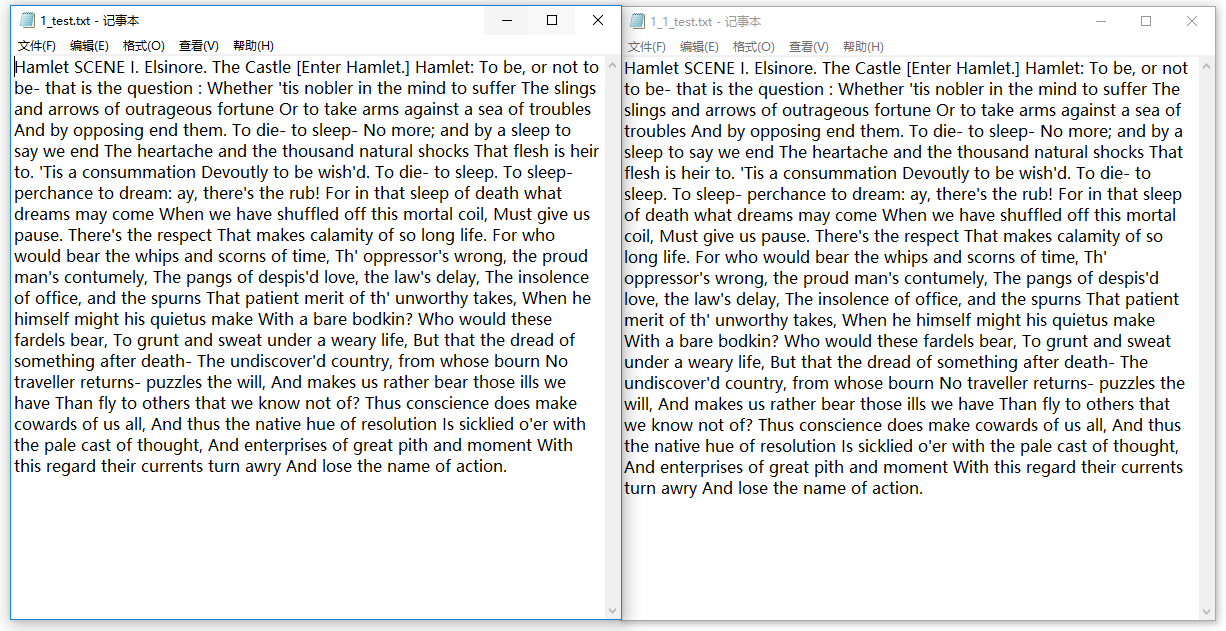
\includegraphics[width=\linewidth]{fig/test.png}
\caption{运行ps3\_tests\_f16.py的结果,可以看出所有测试样例通过}
\label{fig:all}
\end{figure}

\begin{figure}[H]
\centering
\begin{tabular}{cc}
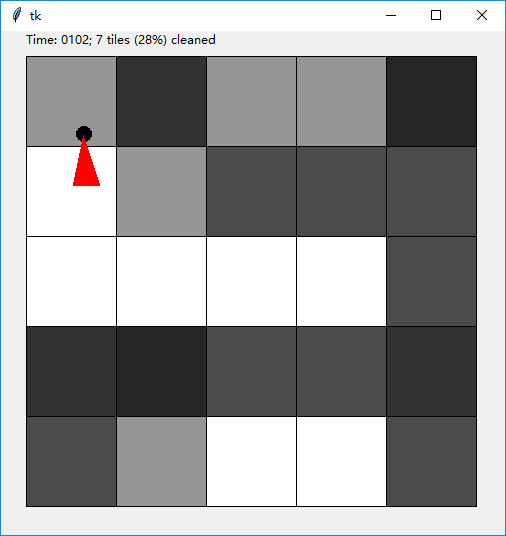
\includegraphics[width=0.4\linewidth]{fig/problem3-1.png}&
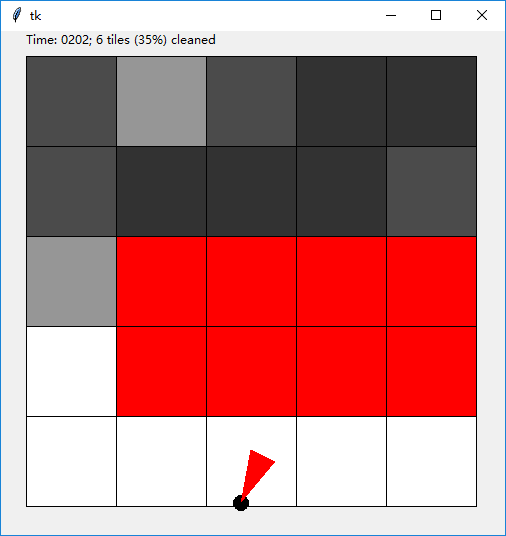
\includegraphics[width=0.4\linewidth]{fig/problem3-2.png}\\
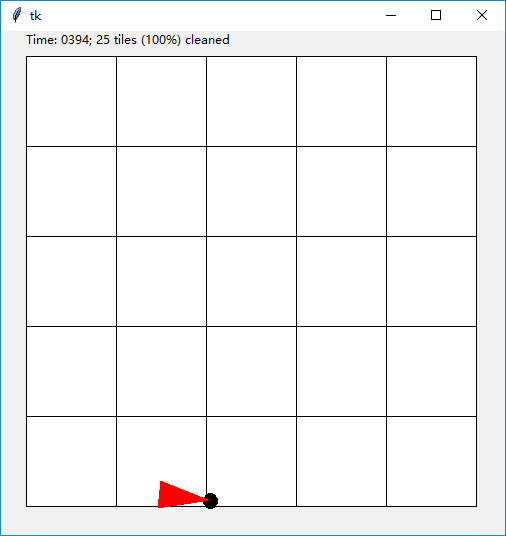
\includegraphics[width=0.4\linewidth]{fig/problem3-3.png}&
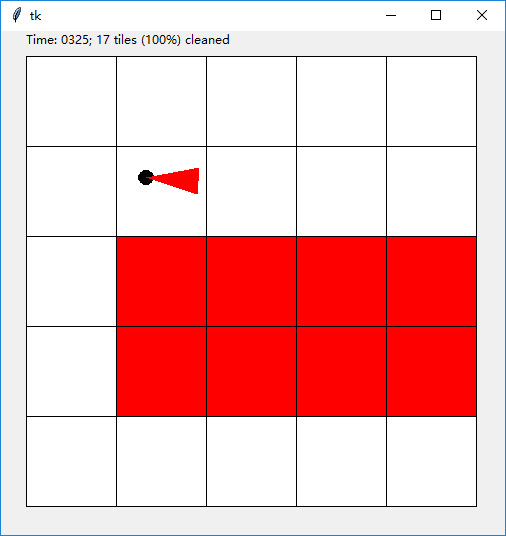
\includegraphics[width=0.4\linewidth]{fig/problem3-4.png}
\end{tabular}
\caption{问题三结果,左侧无家具,右侧有家具。这是运行期间截图,最终都能清理完}
\label{fig:3}
\end{figure}

\begin{figure}[H]
\centering
\begin{tabular}{cc}
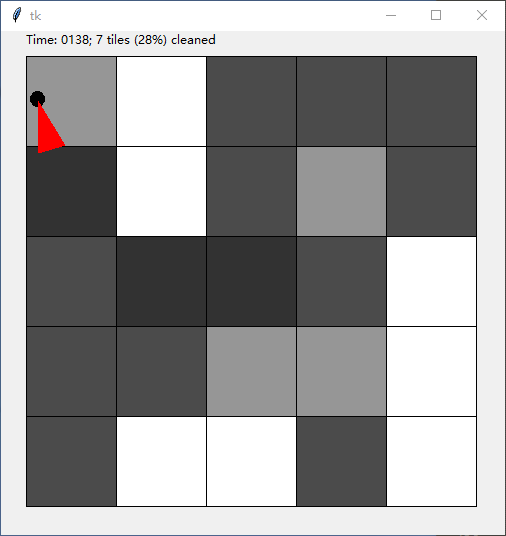
\includegraphics[width=0.4\linewidth]{fig/problem4-1.png}&
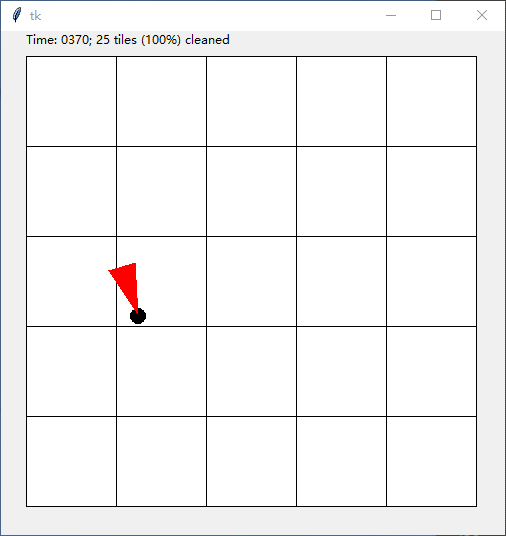
\includegraphics[width=0.4\linewidth]{fig/problem4-2.png}
\end{tabular}
\caption{问题四结果,虽然能够全部清扫完,但明显时间要长很多}
\label{fig:4}
\end{figure}

\begin{figure}[H]
\centering
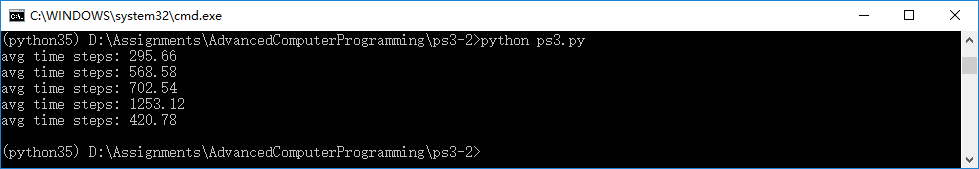
\includegraphics[width=\linewidth]{fig/problem5.png}
\caption{问题五计数结果,明显看出多台机器人一起工作时清理时间最少}
\label{fig:5}
\end{figure}

\begin{figure}[H]
\centering
\begin{tabular}{cc}
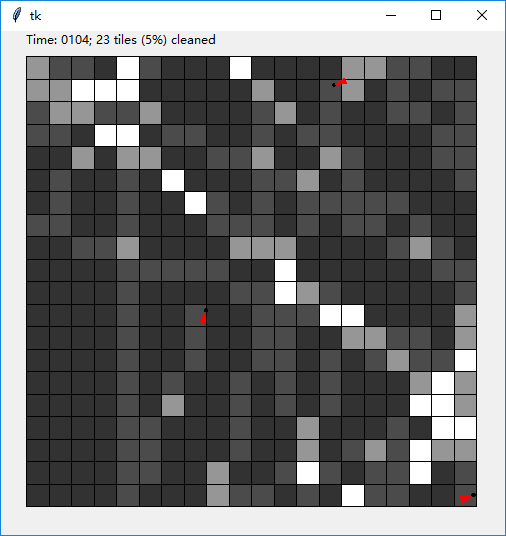
\includegraphics[width=0.4\linewidth]{fig/problem5-1.png}&
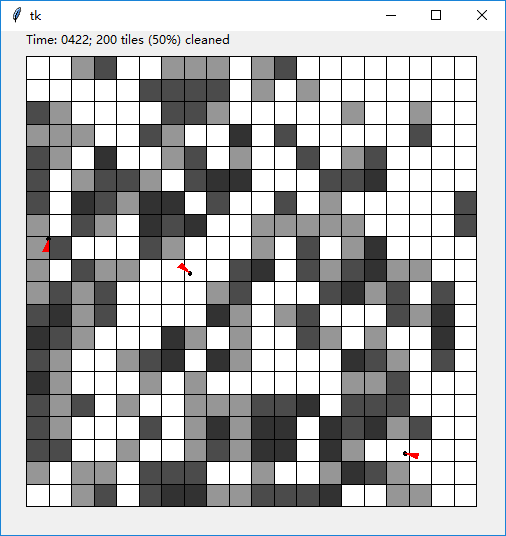
\includegraphics[width=0.4\linewidth]{fig/problem5-2.png}
\end{tabular}
\caption{问题五可视化结果,阈值为50\%清理率}
\label{fig:5v}
\end{figure}

\begin{figure}[H]
\centering
\begin{tabular}{cc}
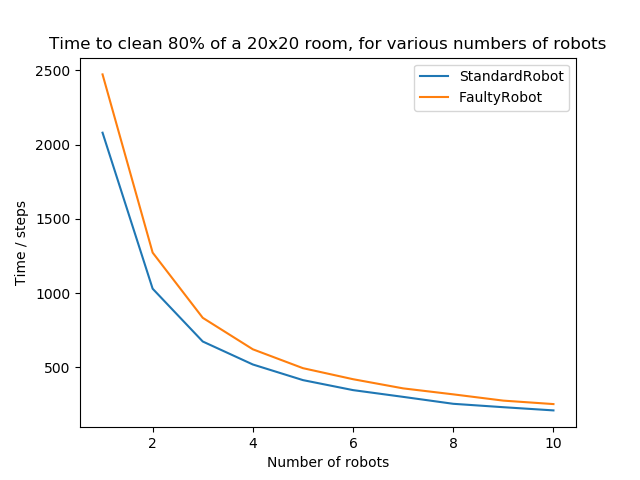
\includegraphics[width=0.5\linewidth]{fig/problem6-1.png}&
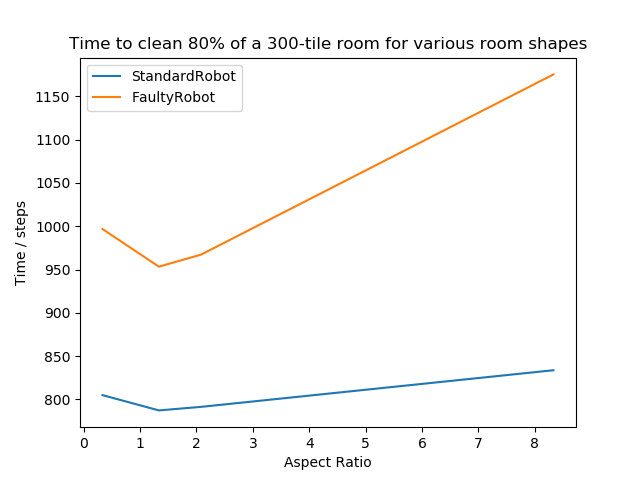
\includegraphics[width=0.5\linewidth]{fig/problem6-2.png}
\end{tabular}
\caption{问题六结果}
\label{fig:6}
\end{figure}

\end{document}

% 实验提交内容
% 邮件主题,作业文件命名规范(学号、姓名)
% 文档pdf格式(问题、求解思路、代码、注释、运行截图)
% 考虑健壮性、可读性
% 极端样例